\section{Introduction} \label{section: introduction}

\subsection{The system for measuring the force applied to the foot when stepping and its importance}
The subject of this project is developing a system to measure and analyze the forces applied to the front and rear of the foot during walking or running. Understanding these ground reaction forces is important for injury prevention, rehabilitation, and athletic performance optimization. Excessive impact forces during foot strike can cause injuries such as stress fractures and plantar fasciitis. On the other hand, optimized foot force patterns can improve efficiency and speed for runners. Currently, force measurements require expensive lab equipment like force plates. This project aims to develop an affordable, wearable sensor system to measure foot forces during real-world activities. Analyzing force data could help identify high-risk movement patterns and guide training improvements. Widespread access to foot force measurement could benefit recreational and competitive athletes as well as clinical populations.

\subsection{The existing systems and specifications}
This project involves developing a wearable system to measure forces on the front and back of the foot during walking and running. These ground reaction forces are important biomechanical markers but currently difficult to monitor outside laboratories. This project aims to create an affordable, portable sensor system to quantify foot forces, using pressure sensors attached to the foot. Measuring foot forces could enable injury prevention and optimization for athletes and clinical populations.

Real world apllications of this system include:
\begin{itemize}
    \item \textbf{Rehabilitation:} foot force measurements could help track recovery progress and identify high-risk movement patterns.
    \item \textbf{Athletic performance optimization:} Optimized foot force patterns can improve efficiency and speed for runners. Measuring foot forces could help identify high-risk movement patterns and guide training improvements.
    \item \textbf{Clinical populations:} foot force measurements could help track recovery progress and identify high-risk movement patterns.
\end{itemize}

Here is some real world examples of the applications of this system:
\begin{figure}[H]
    \centering
    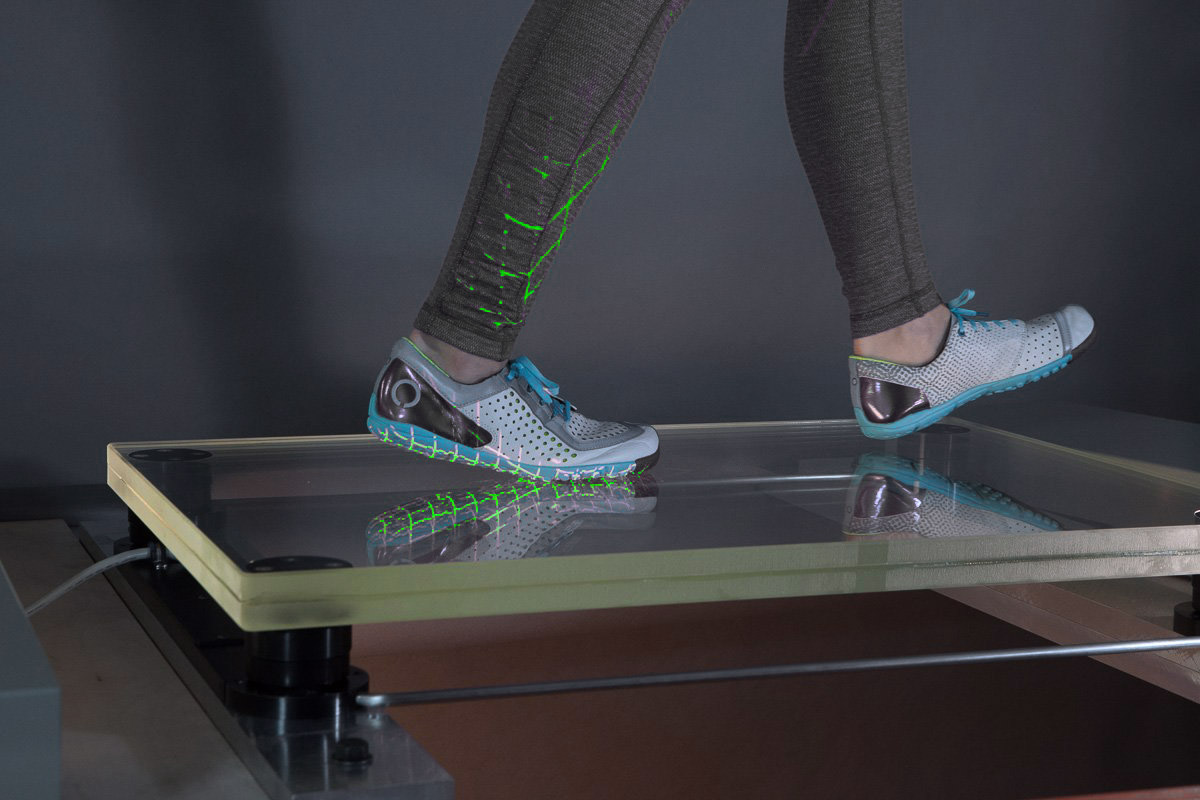
\includegraphics[width=0.8\textwidth]{../Report/Figures/1.Introduction/Force-plate.jpg}
    \caption{A force plate used in a laboratory setting to measure ground reaction forces.}
\end{figure}

\subsection{What we have done}
First we used a matlab code to simulate the input signal of the sensor. Then we designed a circuit to measure the force applied to the sensor. We used LtSpice to simulate the circuit and test it and checked the results.

\subsection{Presentation of information in the rest of the report}
In the next section, we will explain the theoretical background of the project. Then we will explain the circuit design and the simulation results. Finally, we will discuss the results and conclude the project.





